\section{Considerations on Free Surfaces}\label{sec:free-surfaces}

\begin{figure}
    \begin{subfigure}{0.5\linewidth}
        \centering
        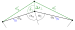
\includegraphics{img/model_development/surface_normal}
        \caption{Normal Direction}
        \label{fig:model_development/surface_normal}
    \end{subfigure}%
    \begin{subfigure}{0.5\linewidth}
        \centering
        \includegraphics{img/model_development/surface_tangential}
        \caption{Tangential Direction}
        \label{fig:model_development/surface_tangential}
    \end{subfigure}
    \caption{Shifting of Surface Nodes}
    \label{fig:surface-node-shifting}
\end{figure}

\begin{equation}
    \SurfaceNormalAngle = \pi - \frac{1}{2} \left(\Upper\SurfaceRadiusAngle + \Lower\SurfaceRadiusAngle\right)
    \label{eq:delta-surface-normal}
\end{equation}

\begin{subequations}
    \begin{equation}
        \Normal\GibbsEnergyStep = \left( \Upper\SurfaceDistance' - \Upper\SurfaceDistance + \Lower\SurfaceDistance' - \Lower\SurfaceDistance \right) \Surface{\InterfaceEnergy}
        \label{eq:gibbs-diff-surface-normal}
    \end{equation}

    with

    \begin{align}
        \Upper\SurfaceDistance' &= \sqrt{\Upper{\SurfaceDistance}^2 + \Normal{\ShiftStep}^2 - 2 \Upper{\SurfaceDistance} \Normal{\ShiftStep} \cos \SurfaceNormalAngle} \\
        \Lower\SurfaceDistance' &= \sqrt{\Lower{\SurfaceDistance}^2 + \Normal{\ShiftStep}^2 - 2 \Lower{\SurfaceDistance} \Normal{\ShiftStep} \cos \SurfaceNormalAngle}
    \end{align}
\end{subequations}

\begin{equation}
    \frac{\partial \GibbsEnergy}{\partial \Normal{\Shift}} = \lim_{\Normal\ShiftStep \rightarrow 0} \frac{\Normal\GibbsEnergyStep}{\Normal\ShiftStep} = -2 \Surface{\InterfaceEnergy} \cos \SurfaceNormalAngle
    \label{eq:gibbs-partial-surface-normal}
\end{equation}

\begin{equation}
    \frac{\partial \Volume}{\partial \Normal{\Shift}} = \frac{1}{2} \left( \Upper\SurfaceDistance + \Lower\SurfaceDistance \right) \sin \SurfaceNormalAngle
    \label{eq:volume-partial-surface-normal}
\end{equation}

\begin{equation}
    \SurfaceTangentAngle = \SurfaceNormalAngle - \frac{\pi}{2}
    \label{eq:delta-surface-tangential}
\end{equation}

\begin{subequations}
    \begin{equation}
        \Tangential\GibbsEnergyStep = \left( \Upper\SurfaceDistance' - \Upper\SurfaceDistance + \Lower\SurfaceDistance' - \Lower\SurfaceDistance \right) \Surface{\InterfaceEnergy}
        \label{eq:gibbs-diff-surface-tangential}
    \end{equation}

    with (note the sign before cosine term)

    \begin{align}
        \Upper\SurfaceDistance' &= \sqrt{\Upper{\SurfaceDistance}^2 + \Tangential{\ShiftStep}^2 + 2 \Upper{\SurfaceDistance} \Tangential{\ShiftStep} \cos \SurfaceTangentAngle} \\
        \Lower\SurfaceDistance' &= \sqrt{\Lower{\SurfaceDistance}^2 + \Tangential{\ShiftStep}^2 - 2 \Lower{\SurfaceDistance} \Tangential{\ShiftStep} \cos \SurfaceTangentAngle}
    \end{align}
\end{subequations}

\begin{equation}
    \frac{\partial \GibbsEnergy}{\partial \Tangential{\Shift}} = \lim_{\Tangential\ShiftStep \rightarrow 0} \frac{\Tangential\GibbsEnergyStep}{\Tangential\ShiftStep} = 0
    \label{eq:gibbs-partial-surface-tangential}
\end{equation}

\begin{equation}
    \frac{\partial \Volume}{\partial \Tangential{\Shift}} = \frac{1}{2} \left( \Lower\SurfaceDistance - \Upper\SurfaceDistance \right) \sin \SurfaceTangentAngle
    \label{eq:volume-partial-surface-tangential}
\end{equation}